\chapter{Erstellen eines Datensatzes}\label{chapter:dataset}
Ein wichtiger Bestandteil beim Entwickeln von künstlichen neuronalen Netzen ist
der unterliegende Datensatz, der zum Trainieren der Parameter der Netze
verwendet wird. Eine Machine-Learning-Modell ist nur so gut wie der verwendete
Datensatz. Dieser muss deshalb eine große Varianz der repräsentierten Daten
besitzen. Das bedeutet, dass ausreichend Einträge vorhanden sein müssen, um das
Netzwerk auf ähnliche, aber unbekannte Probleme vorzubereiten. Ein beliebter
Datensatz ist beispielsweise der MNIST-Datensatz \cite{6296535}, welcher unter
anderem Bilder von handgeschriebenen Ziffern bereitstellt. Anhand des
MNIST-Beispiels bedeutet eine große Varianz, dass eine Ziffer durch viele
verschiedene Bilder repräsentiert wird, die alle eine andere Perspektive des
gleichen Kontexts darstellen.

In diesem Abschnitt soll nun ein Datensatz eingeführt werden, welcher Daten für
die Bewegungserkennung unterstützt. Um diesen Datensatz zu erstellen, muss vorab
geklärt werden, was eine Bewegung eigentlich ist. Betrachtet man einen Punkt im
Raum, dann beschreibt eine Bewegung die Änderung des Ortes eines Objekts über
die Zeit. Bezogen auf den zu erstellenden Datensatz bedeutet dies, dass einfache
Bildaufnahmen von beweglichen (dynamischen) Objekten nicht ausreichen. Um eine
Bewegung aufzuzeichnen, müssen zeitlich aufeinander folgende Bilder aufgenommen
werden, die letzlich Videos darstellen. Da der Datensatz später dazu verwendet
werden soll, um ein neuronales Netz zu trainieren, welches Bewegungen erkennt,
müssen die zu erlernenden Bewegungen auch in diesem Datensatz als Videos
vertreten sein.

Bevor ein Modell für die Bewegungserkennung und -analyse trainiert wird, soll
zusätzlich untersucht werden, ob ein relativ kleiner Datensatz ausreichend ist,
um trotzdem gute Resultate beim Trainieren von neuronalen Netzen zu erzeugen. Da
diese Netze jedoch auf einen vielseitigen Datensatz zurückgreifen müssen, um
entsprechend gute Erkennungsraten zu erzeugen, ist die Idee, diesen kleinen
Datensatz künstlich zu erweitern. Interessant hierbei ist, ob ein künstlich
gedehnter Datensatz genau so gut geeignet ist, wie ein aufwändig erstellter
Datensatz bestehend aus realen Daten. Falls sich das Experiment als erfolgreich
herausstellt, liegt der Vorteil auf der Hand. Nämlich dass künstlich erzeugte
Datensätze wesentlich schneller auszuheben sind als Datensätze mit
ausschließlich realen Daten. Dies würde den Arbeitsaufwand für das Erstellen von
neuen komplexen Datensätzen um ein vielfaches verringern und gleichzeitig den
Fokus auf die eigentliche Forschungsarbeit verbessern.

Nun stellt sich natürlich die Frage, wie ein kleiner Datensatz künstlich
vergrößert werden kann. Künstlich bedeutet hier, dass das Vergrößern des
Datensatzes mithilfe von Algorithmen geschiet und vom Computer anstatt vom
Menschen durchgeführt wird. Eine Möglichkeit ist es, die Daten zu augmentieren.
Dies wird bereits häufig während des Trainings von neuronalen Netzen
durchgeführt, indem simple Transformationen wie Rotation, Translation und
Verzerrung an den Daten durchgeführt werden. Aber auch das Verändern des
Gamma-Wertes eines Bildes reicht in einigen Fällen aus, um eine Variation im
Datensatz künstlich zu erzeugen. Eine weitere Möglichkeit ist es, anderen
neuronalen Netzen diese Arbeit übernehmen zu lassen. Hierbei werden generative
Modelle wie GANs verwendet, um neue, bisher unbekannte Samples eines Datensatzes
zu erzeugen. Auch diese Idee ist nicht neu, jedoch beziehen sich die meisten
Beispiele auf das Generieren von einfachen Bildern. Da es sich bei dem zu
erstellenden Datensatz um Videos handelt, müssen die Techniken auf dieses
Problem angewandt werden. Neben den Inhalt von einzelnen Bildern muss das GAN
als zusätzliche Dimension also die Semantik zwischen einzelnen Frames bzw.
Bildern erlernen und neu generieren können, da es keinen Sinn ergibt, dass der
Kontext pro Videoframe zufällig wechselt. Stattdessen wird gefordert, dass jeder
erzeugte Frame von dem vorherigen abhängt, sodass die Folge der Frames ein
sinnvolles Video ergibt.

\section{Architektur von ViGAN}
In diesem Abschnitt wird die Architektur von ViGAN vorgestellt und die
Idee dahinter erläutert. ViGAN steht für Video-Generative-Adversarial-Network
und dient zum Erzeugen von neuen Videos aus einem bestehendem Datensatz. Gerade
das Erstellen von Videos und das Labeln der Bewegungen nimmt enorm viel Zeit in
Anspruch. Mithilfe von ViGAN soll der Aufwand reduziert werden. Hierbei wird
untersucht, ob ein künstlich erweiterter Datensatz für das Trainieren von
neuronalen Netzen geeignet ist. In Kapitel \ref{chapter:gans} werden
verschiedene GANs und deren Probleme bzw. Vorteile vorgestellt. Aufgrund der
Vorteile von Wasserstein-GANs, nämlich die Interpretationsmöglichkeit des Losses
während des Trainings und die Mode-Collapse-Resistenz, wird dieses als
Grundarchitektur gewählt. Da häufig GANs nur in Verbindung mit einzelnen Bildern
verwendet werden, muss das WGAN entsprechend angepasst werden, um Videos anstatt
von Bildern zu erzeugen. Wie im vorherigen Abschnitt besprochen, ist es wichtig,
dass die Frames des Videos zueinander passen und nicht aus dem Kontext gerissen
werden. Wie in Abbildung \ref{fig:vigan} dargestellt unterscheidet sich ViGAN
nicht allzu sehr vom WGAN. Der größte Unterschied besteht darin, dass
3D-Convolutional-Layer anstelle der 2D-Convolutional-Layer verwendet werden.
Dies ermöglicht nicht nur ein Upsampling des Bildes, sondern auch die Anzahl der
Frames. Die Idee dabei ist, dass das Netzwerk dadurch lernt, zusammenhängende
Frames zu generieren. Als Eingabe wird ein zufälliger Vektor $z$ gewählt. Dann
muss das Netzwerk die eindimensionale Eingabe in eine vierdimensionale Struktur
umwandeln. Dies geschieht beim ViGAN mithilfe eines Fully-Connected-Layers mit
$5 \cdot 6 \cdot 8 \cdot 256$ Neuronen und einem Reshape-Layer, welcher die
Ausgabe des Fully-Connected-Layers in einen 4D-Tensor mit den Dimensionen $(5,
6, 8, 256)$ umstrukturiert. Die erste Dimension beschreibt dabei immer die
Anzahl der Frames, die zweite die Höhe, die dritte die Breite und die vierte die
Anzahl der Farbkanäle. Anschließend wird der Tensor mithilfe eines
Convolutional-Layers vergrößert und die Frameanzahl erhöht. Der Stride beträgt
dabei 2, sodass eine Verdoppelung der Dimensionen stattfindet. Insgesamt werden
vier solcher Schichten hinereinander gereiht. Dabei entsteht ein Ausgabevideo
mit 80 Frames, wobei jeder Frame jeweils $96 \times 128 \times 3$ Pixelwerte
besitzt.

\begin{figure}
    \centering
    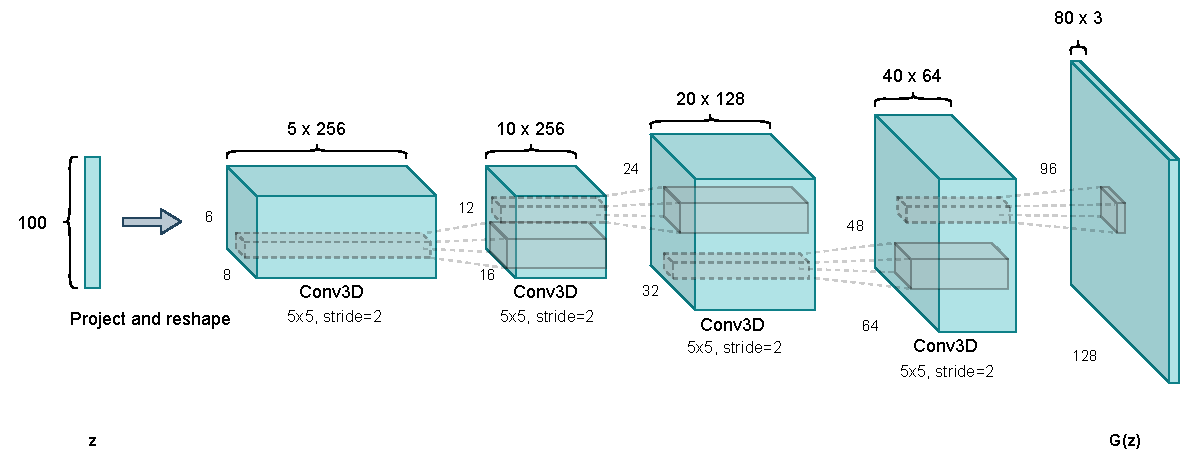
\includegraphics[width=\textwidth]{images/ViGAN.pdf}
    \caption{Architektur von ViGAN. Als Eingabe dient ein zufälliger Vektor $z
    \in \mathbb{R}^{100}$. Dieser wird anschließend in fünf $6 \times 8 \times
    256$ Features umgewandelt. Um die relativ kleinen Frames in eine größere
    Auflösung zu skalieren, werden vier 3D-Convolutional-Layer verwendet. Jedes
    dieser Schichten verwendet eine Kernelgröße von $5 \times 5 \times 5$ und
    einen Stride von 2.  Insgesamt ergibt sich also ein Stride von $2^4 = 16$,
    sodass die Eingabegröße von $5 \times 6 \times 8 \times 256$ auf 80x96x128x3
    hochskaliert wird.}
    \label{fig:vigan}
\end{figure}

\section{Experimente und Diskussion der Ergebnisse}
Um die Brauchbarkeit vom ViGAN zu testen, werden einige Experimente durchgeführt, die 